\documentclass{zusammenfassung}
\usepackage{array}
\usepackage{booktabs}
\usepackage{color}
\usepackage{colortbl}
\usepackage{xstring}
\usepackage{intcalc}
\usepackage{alphalph}
\usepackage{algpseudocode}
\usepackage[misc]{ifsym}
\graphicspath{ {./illustrationen/} }
\setmonofont{Linux Libertine Mono}
\usetikzlibrary{positioning}
\usetikzlibrary{arrows}

\begin{document}
\maketitle{Klasse 6/7}{16. Juni 2015}{2014/2015}

Für diesen Zirkel haben Graphen zwischen zwei Knoten höchstens eine Kante. Nicht erlaubt ist also folgender Graph:

\begin{center}
	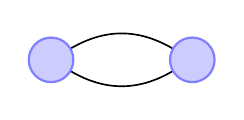
\begin{tikzpicture}
		[inner sep=2mm,
			every node/.style={circle,draw=blue!50,fill=blue!20,thick},
			connect/.style={semithick},
		node distance=1.2]
		\node (n1) {};
		\node (n2) [right=of n1] {}
		  edge [connect,bend right] (n1)
			edge [connect,bend left] (n1);
	\end{tikzpicture}
\end{center}

Ein \emph{Kreis} in einem Graphen ist ein Kantenzug mit gleichem Anfangs- wie Endpunkt, der keine Kante mehrfach benutzt.
Ein \emph{Wald} ist ein Graph, der keine Kreise enthält. Ein \emph{Baum} schließlich ist ein zusammenhängender Wald.

\begin{aufgabe}
	Welche der folgenden Graphen sind Wälder? Welche sind Bäume?
	\begin{center}
		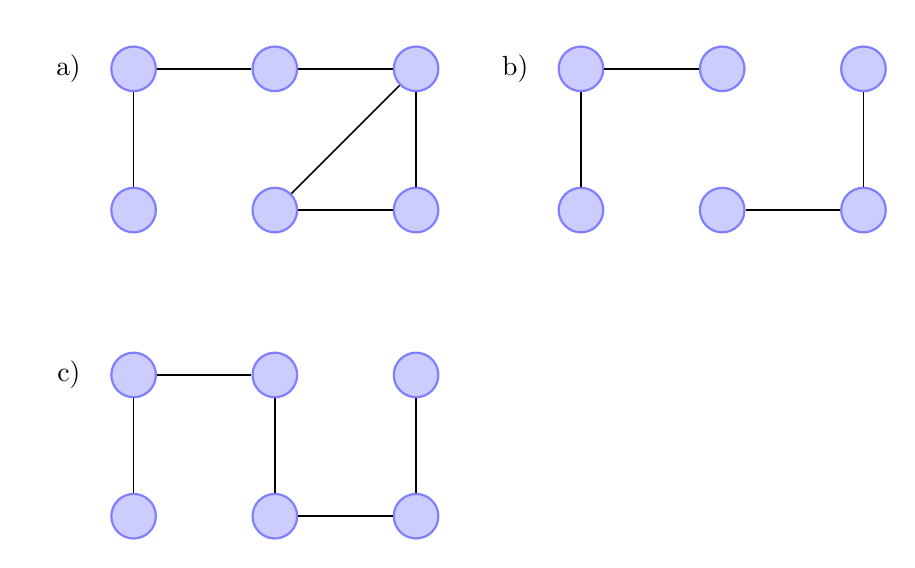
\begin{tikzpicture}
			[inner sep=2mm,
			 every node/.style={circle,draw=blue!50,fill=blue!20,thick},
			 connect/.style={semithick},
		   node distance=1.2]
			\node (n1) {};
			\node (n2) [below=of n1] {}
			  edge [connect] (n1);
			\node (n3) [right=of n1] {}
			  edge [connect] (n1);
			\node (n4) [right=of n2] {};
			\node (n5) [right=of n3] {}
				edge [connect] (n3)
				edge [connect] (n4);
			\node (n6) [right=of n4] {}
			  edge [connect] (n5)
				edge [connect] (n4);
			\node [left=0 of n1,draw=none,fill=none] {a)};

			\node (b1) [right=1.5 of n5] {};
			\node (b2) [below=of b1] {}
			  edge [connect] (b1);
			\node (b3) [right=of b1] {}
			  edge [connect] (b1);
			\node (b4) [right=of b2] {};
			\node (b5) [right=of b3] {};
			\node (b6) [right=of b4] {}
			  edge [connect] (b5)
				edge [connect] (b4);
			\node [left=0 of b1,draw=none,fill=none] {b)};

			\node (c1) [below=1.5 of n2] {};
			\node (c2) [below=of c1] {}
			  edge [connect] (c1);
			\node (c3) [right=of c1] {}
			  edge [connect] (c1);
			\node (c4) [right=of c2] {}
			  edge [connect] (c3);
			\node (c5) [right=of c3] {};
			\node (c6) [right=of c4] {}
			  edge [connect] (c5)
				edge [connect] (c4);
			\node [left=0 of c1,draw=none,fill=none] {c)};
	  \end{tikzpicture}
  \end{center}
\end{aufgabe}

\pagebreak

Ein \emph{Spannbaum} in einem Graphen ist ein Baum, der alle Knoten des Graphen enthält.

\begin{aufgabe}
	Finde Spannbäume in folgenden Graphen:
	\begin{center}
		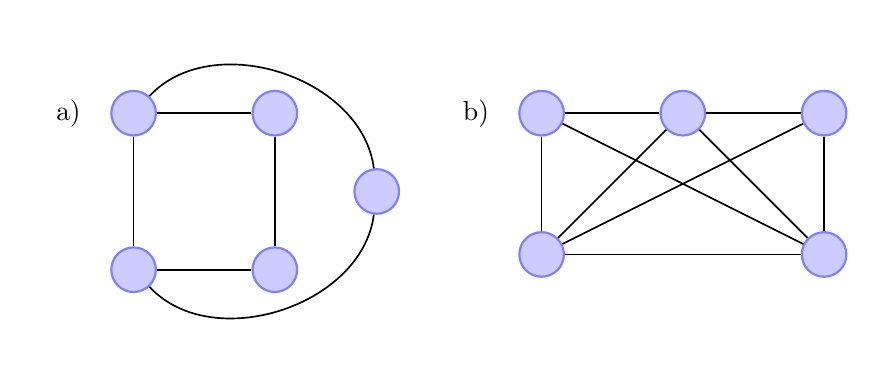
\begin{tikzpicture}
			[inner sep=2mm,
			 every node/.style={circle,draw=blue!50,fill=blue!20,thick},
			 connect/.style={semithick},
		   node distance=1.2]
			\node (e1) {};
			\node (e1a) [below=0.4 of e1,draw=none,fill=none] {};
			\node (e2) [below=0.4 of e1a] {}
			  edge [connect] (e1);
			\node (e3) [right=of e1] {}
			  edge [connect] (e1);
			\node (e4) [right=of e2] {}
			  edge [connect] (e2)
				edge [connect] (e3);
			\node (e5) [right=0.7 of e3,draw=none,fill=none] {};
			\node (e6) [below=0.4 of e5] {}
			  edge [connect,bend right=65] (e1)
				edge [connect,bend left=65] (e2);
		  \node [left=0 of e1,draw=none,fill=none] {a)};

			\node (f1) [right=1.5 of e5] {};
			\node (f2) [right=of f1] {}
			  edge [connect] (f1);
			\node (f3) [right=of f2] {}
			  edge [connect] (f2);
			\node (f4) [below=of f1] {}
			  edge [connect] (f1)
				edge [connect] (f2)
				edge [connect] (f3);
			\node (f5) [below=of f3] {}
			  edge [connect] (f1)
				edge [connect] (f2)
				edge [connect] (f3)
				edge [connect] (f4);
			\node [left=0 of f1,draw=none,fill=none] {b)};
		\end{tikzpicture}
	\end{center}
\end{aufgabe}

\begin{aufgabe}
	Warum hat jeder zusammenhängende Graph einen Spannbaum?
\end{aufgabe}

Eine \emph{Kostenfunktion} ordnet jeder Kante $e$ einen Wert $c_e$ zu. Wir wollen einen Spannbaum mit minimalen Kosten (also einen
\emph{minimalen Spannbaum}) finden. Man kann sich die Situation folgendermaßen vorstellen: Die Knoten des Graphen sind Städte, die
alle an ein gemeinsames Stromnetz angebunden werden sollen. Die Kosten einer Kante sind die Kosten für die jeweilige Verbindung
der beiden Städte. Wir wollen alle Städte miteinander verbinden, und das so günstig wie möglich. Dieses Ziel wird mit einem
minimalen Spannbaum erreicht.

Wenn nichts anderes gesagt wird, soll hier $n$ die Anzahl der Knoten und $m$ die Anzahl der Kanten bezeichnen. Wir beginnen mit
zwei Beobachtungen:

\begin{itemize}
	\item \emph{Falls $m\geq n$ ist, gibt es mindestens einen Kreis.} Diese Aussage wird mit einem Beweisverfahren begründet, das
		sich \emph{vollständige Induktion} nennt. Die Idee dabei ist, dass man die Behauptung für kleine Zahlen leicht beweisen kann
		und dass man aus der Aussage für eine Zahl $n$ auch schon auf die Aussage für $n+1$ schließen kann. Dann kann man sich
		sozusagen "`hochhangeln"': Die Aussage gilt für $n=1$, also muss sie auch für $n=1+1=2$ gelten, also auch für $n=2+1=3$ und so
		weiter. Dieses Verfahren wird in der Mathematik sehr häufig eingesetzt und ist meistens nützlich, wenn Aussagen über alle
		natürlichen Zahlen bewiesen werden sollen.

		Wie sieht das in unserer Situation konkret aus? Nun, für $n=1$ und $n=2$ tritt der Fall $m\geq n$ überhaupt nicht auf, da
		keine Kante von einem Knoten zu sich selbst und keine zwei Kanten zwischen zwei verschiedenen Knoten verlaufen dürfen. Die
		einzige Möglichkeit, wie $m\geq n$ für $n=3$ erfüllt sein kann, ist folgende:
		\enlargethispage{2.8cm}
		\begin{center}
			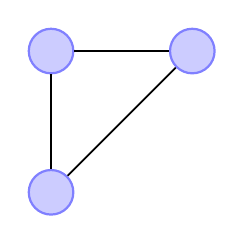
\begin{tikzpicture}
				[inner sep=2mm,
					every node/.style={circle,draw=blue!50,fill=blue!20,thick},
					connect/.style={semithick},
				node distance=1.2]
				\node (a1) {};
				\node (a2) [below=of a1] {}
				  edge [connect] (a1);
				\node (a3) [right=of a1] {}
					edge [connect] (a1)
					edge [connect] (a2);
			\end{tikzpicture}
		\end{center}
		In diesem Graphen gibt es offensichtlich einen Kreis.
		\pagebreak

		Nun nehmen wir an, dass die Aussage für Graphen mit $n-1$ Knoten schon wahr ist und wir einen Graphen $G$ mit $n$ Knoten und 
		$m\geq n$ Kanten gegeben haben. Wir müssen jetzt zeigen, dass $G$ einen Kreis hat. Angenommen, das wäre nicht der Fall. Dann
		existiert ein Knoten vom Grad $1$. (Man kann nämlich von einem beliebigen Knoten entlang einem beliebigen Kantenzug loslaufen.
		Wenn man darauf achtet, keine Kante doppelt zu benutzen, dann kommt man schließlich an einem Knoten an, von dem aus man nicht
		weiterlaufen kann. Da es keinen Kreis gibt, muss das bedeuten, dass die einzige Kante, die an den Knoten grenzt, diejenige
		ist, mit der man in den Knoten hineingelaufen ist. Wir haben also einen Knoten vom Grad $1$ gefunden.) Der Graph $G'$, der
		entsteht, wenn man diesen Knoten und seine Kante aus $G$ herausnimmt, hat $n-1$ Knoten und $m-1$ Kanten und daher einen Kreis.

	\item \emph{Falls $m\leq n-2$ ist, ist der Graph unzusammenhängend.} Auch diese Aussage wird mit vollständiger Induktion
		bewiesen: Für $n=1$ kann nicht $m\leq n-2$ sein, und für $n=2$ und $m=0$ ist es klar, dass der Graph nicht zusammenhängt. Im
		allgemeinen Fall haben wir wieder einen Graphen $G$ mit $m\leq n-2$ gegeben und nehmen an, er wäre zusammenhängend. Indem wir
		jeweils eine Kante aus jedem auftretenden Kreis entfernen, bleibt der Graph zusammenhängend und wird kreisfrei. Die Bedingung
		$m\leq n-2$ bleibt natürlich auch wahr, da $m$ ja nur kleiner wird, wenn man Kanten entfernt. Daher existiert wieder ein
		Knoten vom Grad $1$, wie vorher ist der Graph $G'$ unzusammenhängend, und damit ist auch $G$ unzusammenhängend.
\end{itemize}

\begin{aufgabe}
	Beweise, dass jeder Spannbaum in einem Graph mit $n$ Knoten genau $n-1$ Kanten haben muss.
\end{aufgabe}

Es gibt jetzt eine weitere Beobachtung: Für einen minimalen Spannbaum $T$ gelten folgende Aussagen:
\begin{itemize}
	\item Falls $e$ eine Kante ist, die nicht in $T$ liegt, dann hat $T+e$ einen Kreis $K$ und $e$ ist die teuerste Kante auf $K$.
	\item Falls $e$ eine Kante in $T$ ist, dann hat $T-e$ zwei Komponenten und $e$ ist die billigste Kante, die diese beiden
		Komponenten verbindet.
\end{itemize}

\pagebreak

Diese Beobachtung führt zu folgendem Algorithmus:

\renewcommand{\algorithmicrequire}{\textbf{Eingabe:}}
\renewcommand{\algorithmicensure}{\textbf{Ausgabe:}}
\begin{algorithmic}
	\Require Graph $G$ mit Kostenfunktion
	\Ensure Minimaler Spannbaum $T$ in $G$
	\State $S\gets\text{alle Knoten, keine Kanten}$, $T\gets G$
	\While{$S\neq T$}
		\State Wende eine der folgenden Regeln an:
		\State $\bullet$ \emph{Regel 1:}\enskip\begin{minipage}[t]{0.7\textwidth}Wähle Komponente $C$ von $S$ und Kante $e\in T$, 
		  $e\notin S$, die aus $C$ hinausführt und unter diesen Kanten minimales Gewicht hat. Setze $S\gets S+e$.\\[-1ex]\end{minipage}
		\State $\bullet$ \emph{Regel 2:}\enskip\begin{minipage}[t]{0.7\textwidth}Wähle Kreis $K$ von $T$ und Ecke $e\in K$, $e\notin
			S$ mit maximalem Gewicht. Setze $T\gets T-e$.\end{minipage}
	\EndWhile
	\State \Return T
\end{algorithmic}

Nun muss man nur noch überprüfen, dass dieser Algorithmus tatsächlich korrekt arbeitet. Dazu überlegt man sich, dass in jedem
Schritt ein minimaler Spannbaum existiert, der "`zwischen"' $S$ und $T$ liegt. Wenn am Ende dann $S=T$ ist, dann muss $T$ (bzw.
$S$) also schon selbst ein minimaler Spannbaum sein.

\pagebreak

\begin{aufgabe}
	Finde minimale Spannbäume in folgenden Graphen:
	\begin{center}
		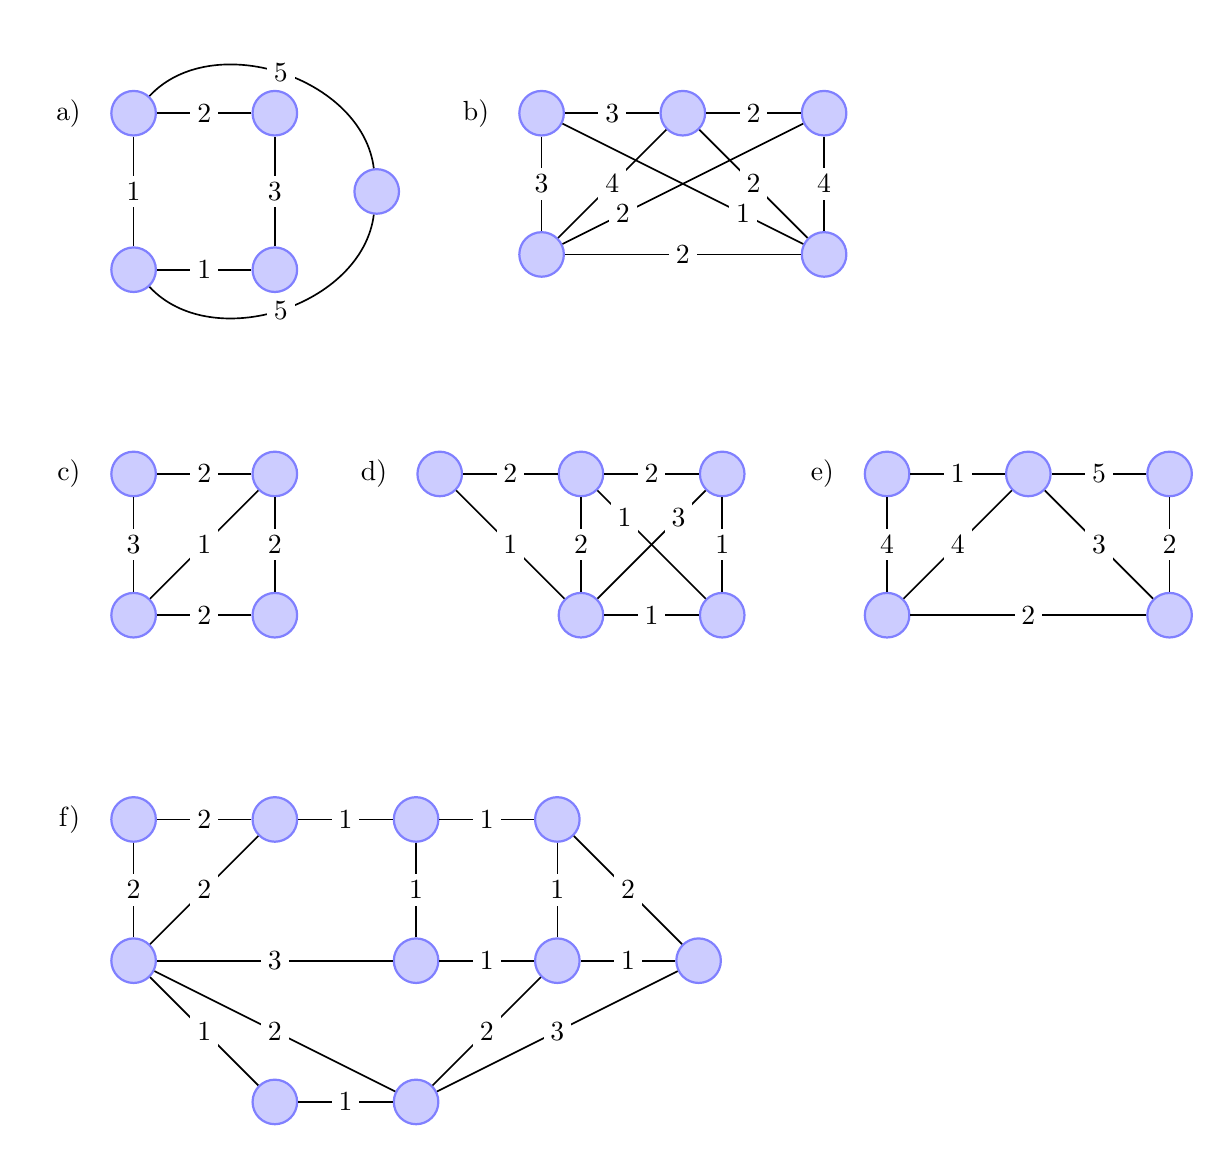
\begin{tikzpicture}
			[inner sep=2mm,
			 every node/.style={circle,draw=blue!50,fill=blue!20,thick},
			 connect/.style={semithick},
			 label/.style={rectangle,fill=white,draw=none,inner sep=.25em},
		   node distance=1.2]
			\node (e1) {};
			\node (e1a) [below=0.4 of e1,draw=none,fill=none] {};
			\node (e2) [below=0.4 of e1a] {}
			edge [connect] node [label] {1} (e1);
			\node (e3) [right=of e1] {}
			edge [connect] node [label] {2} (e1);
			\node (e4) [right=of e2] {}
			edge [connect] node [label] {1} (e2)
			edge [connect] node [label] {3} (e3);
			\node (e5) [right=0.7 of e3,draw=none,fill=none] {};
			\node (e6) [below=0.4 of e5] {}
			edge [connect,bend right=65] node [label] {5} (e1)
			edge [connect,bend left=65] node [label] {5} (e2);
		  \node [left=0 of e1,draw=none,fill=none] {a)};

			\node (f1) [right=1.5 of e5] {};
			\node (f2) [right=of f1] {}
			edge [connect] node [label] {3} (f1);
			\node (f3) [right=of f2] {}
			edge [connect] node [label] {2} (f2);
			\node (f4) [below=of f1] {}
			edge [connect] node [label] {3} (f1)
			edge [connect] node [label] {4} (f2)
			edge [connect] node [label,near start] {2} (f3);
			\node (f5) [below=of f3] {}
			edge [connect] node [label,near start] {1} (f1)
			edge [connect] node [label] {2} (f2)
			edge [connect] node [label] {4} (f3)
			edge [connect] node [label] {2} (f4);
			\node [left=0 of f1,draw=none,fill=none] {b)};

			\node (g1) [below=2 of e2] {};
			\node (g2) [below=of g1] {}
			  edge [connect] node [label] {3} (g1);
			\node (g3) [right=of g1] {}
			  edge [connect] node [label] {2} (g1)
				edge [connect] node [label] {1} (g2);
			\node (g4) [right=of g2] {}
			  edge [connect] node [label] {2} (g3)
				edge [connect] node [label] {2} (g2);
			\node [left=0 of g1,draw=none,fill=none] {c)};

			\node (h1) [right=1.5 of g3] {};
			\node (h2) [right=of h1] {}
			  edge [connect] node [label] {2} (h1);
			\node (h3) [below=of h2] {}
			  edge [connect] node [label] {1} (h1)
				edge [connect] node [label] {2} (h2);
			\node (h4) [right=of h2] {}
			  edge [connect] node [label] {2} (h2)
				edge [connect] node [label,near start] {3} (h3);
			\node (h5) [right=of h3] {}
			  edge [connect] node [label] {1} (h3)
				edge [connect] node [label] {1} (h4)
				edge [connect] node [label,near end] {1} (h2);
			\node [left=0 of h1,draw=none,fill=none] {d)};

			\node (i1) [right=1.5 of h4] {};
			\node (i2) [right=of i1] {}
			  edge [connect] node [label] {1} (i1);
			\node (i3) [right=of i2] {}
			  edge [connect] node [label] {5} (i2);
			\node (i4) [below=of i1] {}
			  edge [connect] node [label] {4} (i1)
				edge [connect] node [label] {4} (i2);
			\node (i5) [below=of i3] {}
			  edge [connect] node [label] {3} (i2)
				edge [connect] node [label] {2} (i3)
				edge [connect] node [label] {2} (i4);
			\node [left=0 of i1,draw=none,fill=none] {e)};

			\node (j1) [below=2 of g2] {};
			\node (j2) [right=of j1] {}
			  edge [connect] node [label] {2} (j1);
			\node (j3) [right=of j2] {}
			  edge [connect] node [label] {1} (j2);
			\node (j4) [right=of j3] {}
			  edge [connect] node [label] {1} (j3);
			\node (j5) [below=of j1] {}
			  edge [connect] node [label] {2} (j1)
				edge [connect] node [label] {2} (j2);
			\node (j6) [below=of j3] {}
			  edge [connect] node [label] {1} (j3)
				edge [connect] node [label] {3} (j5);
			\node (j7) [below=of j4] {}
			  edge [connect] node [label] {1} (j4)
				edge [connect] node [label] {1} (j6);
			\node (j8) [right=of j7] {}
			  edge [connect] node [label] {2} (j4)
				edge [connect] node [label] {1} (j7);
			\node (j9) [below=of j6] {}
			  edge [connect] node [label] {2} (j5)
				edge [connect] node [label] {2} (j7)
				edge [connect] node [label] {3} (j8);
			\node (j10)[left=of j9] {}
			  edge [connect] node [label] {1} (j5)
				edge [connect] node [label] {1} (j9);
			\node [left=0 of j1,draw=none,fill=none] {f)};
		\end{tikzpicture}
	\end{center}
\end{aufgabe}

\end{document}
